\documentclass[aps,rmp, twocolumn]{revtex4}
%\documentclass[a4paper,10pt]{scrartcl}
%\documentclass[aps,rmp,twocolumn]{revtex4}

\usepackage[utf8]{inputenc}
\usepackage{amsmath,graphicx}
\usepackage{color}
\usepackage{booktabs}
%\usepackage{cite}

\newcommand{\bq}{\begin{equation}}
\newcommand{\eq}{\end{equation}}
\newcommand{\bn}{\begin{eqnarray}}
\newcommand{\en}{\end{eqnarray}}
\newcommand{\Richard}[1]{{\color{red}Richard: #1}}
\newcommand{\gene}[1]{{\it #1}}
\newcommand{\mat}[1]{{\bf #1}}
\newcommand{\vecb}[1]{{\bf #1}}
\newcommand{\abet}{\mathcal{A}}
\newcommand{\eqp}{p}
\newcommand{\LH}{\mathcal{L}}


\begin{document}
\title{Evolutionary rates of SARS-CoV-2}
\author{Richard A.~Neher}
\date{\today}
\maketitle

Since its emergence in late 2019, SARS-CoV-2 has displayed a discontinuous pattern of evolution with large unobserved jumps in sequence space giving rise to phylogenetically distinct variants \citep{hodcroft_spread_2021,volz_assessing_2021,tegally_detection_2021,faria_genomics_2021,naveca_covid-19_2021,viana_rapid_2022}.
Many of these variants spread considerably faster and quickly displaced the resident variants either because of intrinsically increased transmissibility, evasion of prior immunity in the population, or a combination of both.
Variants of Concern or Interest were designated by the WHO and labeled by Greek letters \citep{konings_sars-cov-2_2021}.
The branches leading to these variants are characterized by many amino acid changing mutations that often cluster in the S1 domain of the spike protein \citep{kistler_rapid_2022}.
This pattern of rapid non-synonymous evolution in viral surface proteins that interact with the host cells in common among many RNA viruses and for example well studied in influenza virus A evolution \citep{bhatt_genomic_2011,strelkowa_clonal_2012}.

In contrast to influenza virus evolution, the evolution of SARS-CoV-2 has been characterized by unusually large jumps in sequence space.
New variants with 10s of previously unobserved mutations emerged suddenly without intermediate genomes being observed, most dramatically with the emergence of Omicron in later 2021 \citep{viana_rapid_2022}.
The pre-dominant hypothesis for this cryptic emergence of highly mutated, transmissible and immune evasive variants are chronic infections that are frequently observed in patients with impaired immune systems, either through HIV-1 infection \citep{cele_sars-cov-2_2022} or medical intervention \citep{choi_persistence_2020,kemp_sars-cov-2_2021}.
Onward transmission from such chronic infections has also been documented \citep{gonzalez-reiche_intrahost_2022}.
However, to date there is no direct evidence for the emergence of any variant and the degree to which chronic infections might have contributed is a matter of debate.
The case for chronic infection being an important contributor is strongest for the variants Alpha and Omicron
\citep{hill_origins_2022}.

Here, we investigate the rate at which the SARS-CoV-2 genome changes within variants and compare this rate to the rate at which the variants themselves accumulate differences relative to reference sequence.
This comparison reveals a clear dichotomy between slow within-variant evolution and rapid adaptive evolution giving rise to new variants.
The rate of synonymous changes between and within variants agrees, while the non-synonymous rate within variants is far below the between variant rate.
Early variants display more rapid non-synonymous evolution that later variants.

\section*{Results}

Traditionally, evolutionary rates and divergence times are estimates using phylogenetic frameworks for heterochronously sampled sequences.
The volume and heterogeneity of SARS-CoV-2 data, however, mean that one has to dramatically down-sample the data and remove many low quality sequences that would otherwise fatally distort the analysis.

To circumvent many of the above mentioned problems and still use the majority of the available data, we use a combination of automated filtering and robust procedures to analyze the evolutionary patterns.
We first use Nextclade \citep{aksamentov_nextclade_2021} to assign all sequences to one of the Nextstrain \citep{hadfield_nextstrain_2018} clades and analyze each clade separately.
These clades represent well defined groups of sequences with little non-vertical evolution within them.
Furthermore, we define a ``founder'' genotype for each clade and exclude any sequence that does not have the full set of mutations relative to the reference sequence Wuhan/Hu-1.
This filtering removes most incomplete sequences as well as sequences where amplicon drop-out are back-filled with reference sequence.
For this reduced set of sequences, we determine the mutations they carry on top of the founder genotype.
The latter step is done for nucleotide changes as well as for amino acid changes.

Within each clade, the number of mutations is expected to increase linearly in time and the variation around this mean would, in an ideal case, obey Poisson statistics.
To further exclude outliers, we perform a simple linear regression of the number of ``intra-clade'' mutations against time and remove sequences whose deviation from the linear fit exceeds twice the variance by 3.

After removing these outliers, we now bin the data by calendar week and determine the mean and standard deviation in each bin.
Evolutionary rate and putative emergence date of the variant are then estimated by weighted linear regression where each bin is weighted with the fourth root of the number of sequences in the bins.
The exact functional form of this weighing does not have a big influence on the results, but a strongly sublinear weighing helps to counter the large variation in sequencing effort and the natural imbalance due to the fact that few sequences are available early.

Due to shared ancestry, a divergence (or root-to-tip) regression against time is not a suitable method to determine the evolutionary rate.
However, in the case of rapidly expanding variants we typically observe a large number of independent lineages emanating from a basal polytomy.
Along each of these lineages, mutation accumulation is independent and divergence increase allows to estimate the rate.
Fig.~\ref{fig:rate_alpha} shows the increasing intra-clade divergence for clade 20I corresponding to VoC Alpha.

\begin{figure*}[tb]
    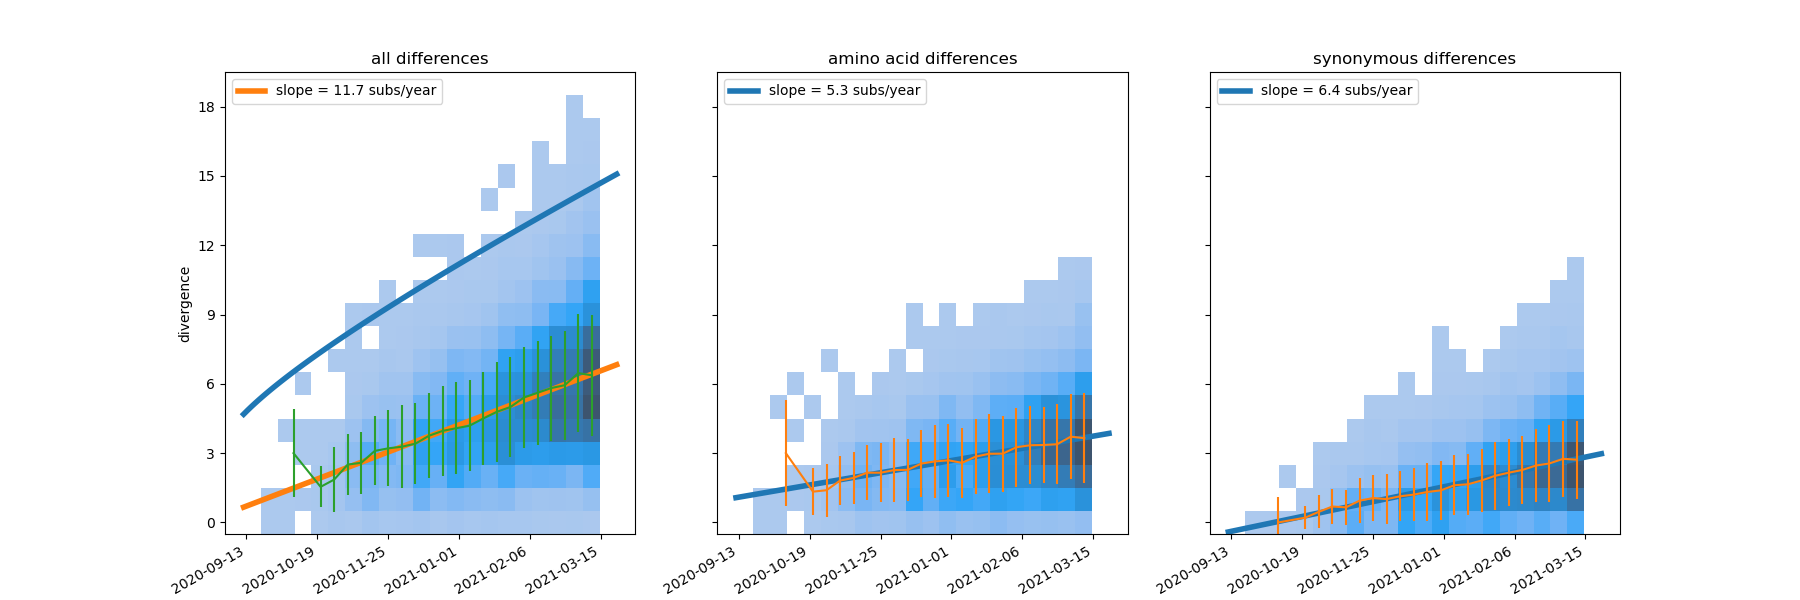
\includegraphics[width=\textwidth]{figures/20I_rtt.png}
    \caption{{\bf Divergence increases linearly with time (20I (Alpha)).} Each panel shows the number of within-clade mutations (total (A), amino acid changing (B), synonymous (C)) as a function of time.
    The blue line in panel A indicates the divergence cut-off, panels B\&C only show sequences that pass the divergence filter. Each panel also shows mean $\pm$ standard deviation and a weighted linear fit.
    \label{fig:rate_alpha}}
\end{figure*}

For almost all major Nextstrain clades, the average divergence increases linearly in time (similar patterns as Fig.~\ref{fig:rate_alpha}) allowing us to estimate clade specific evolutionary rates for amino acid and silent changes.
These rates are summarized in Fig.~\ref{fig:rate_summary}.

\begin{figure*}
    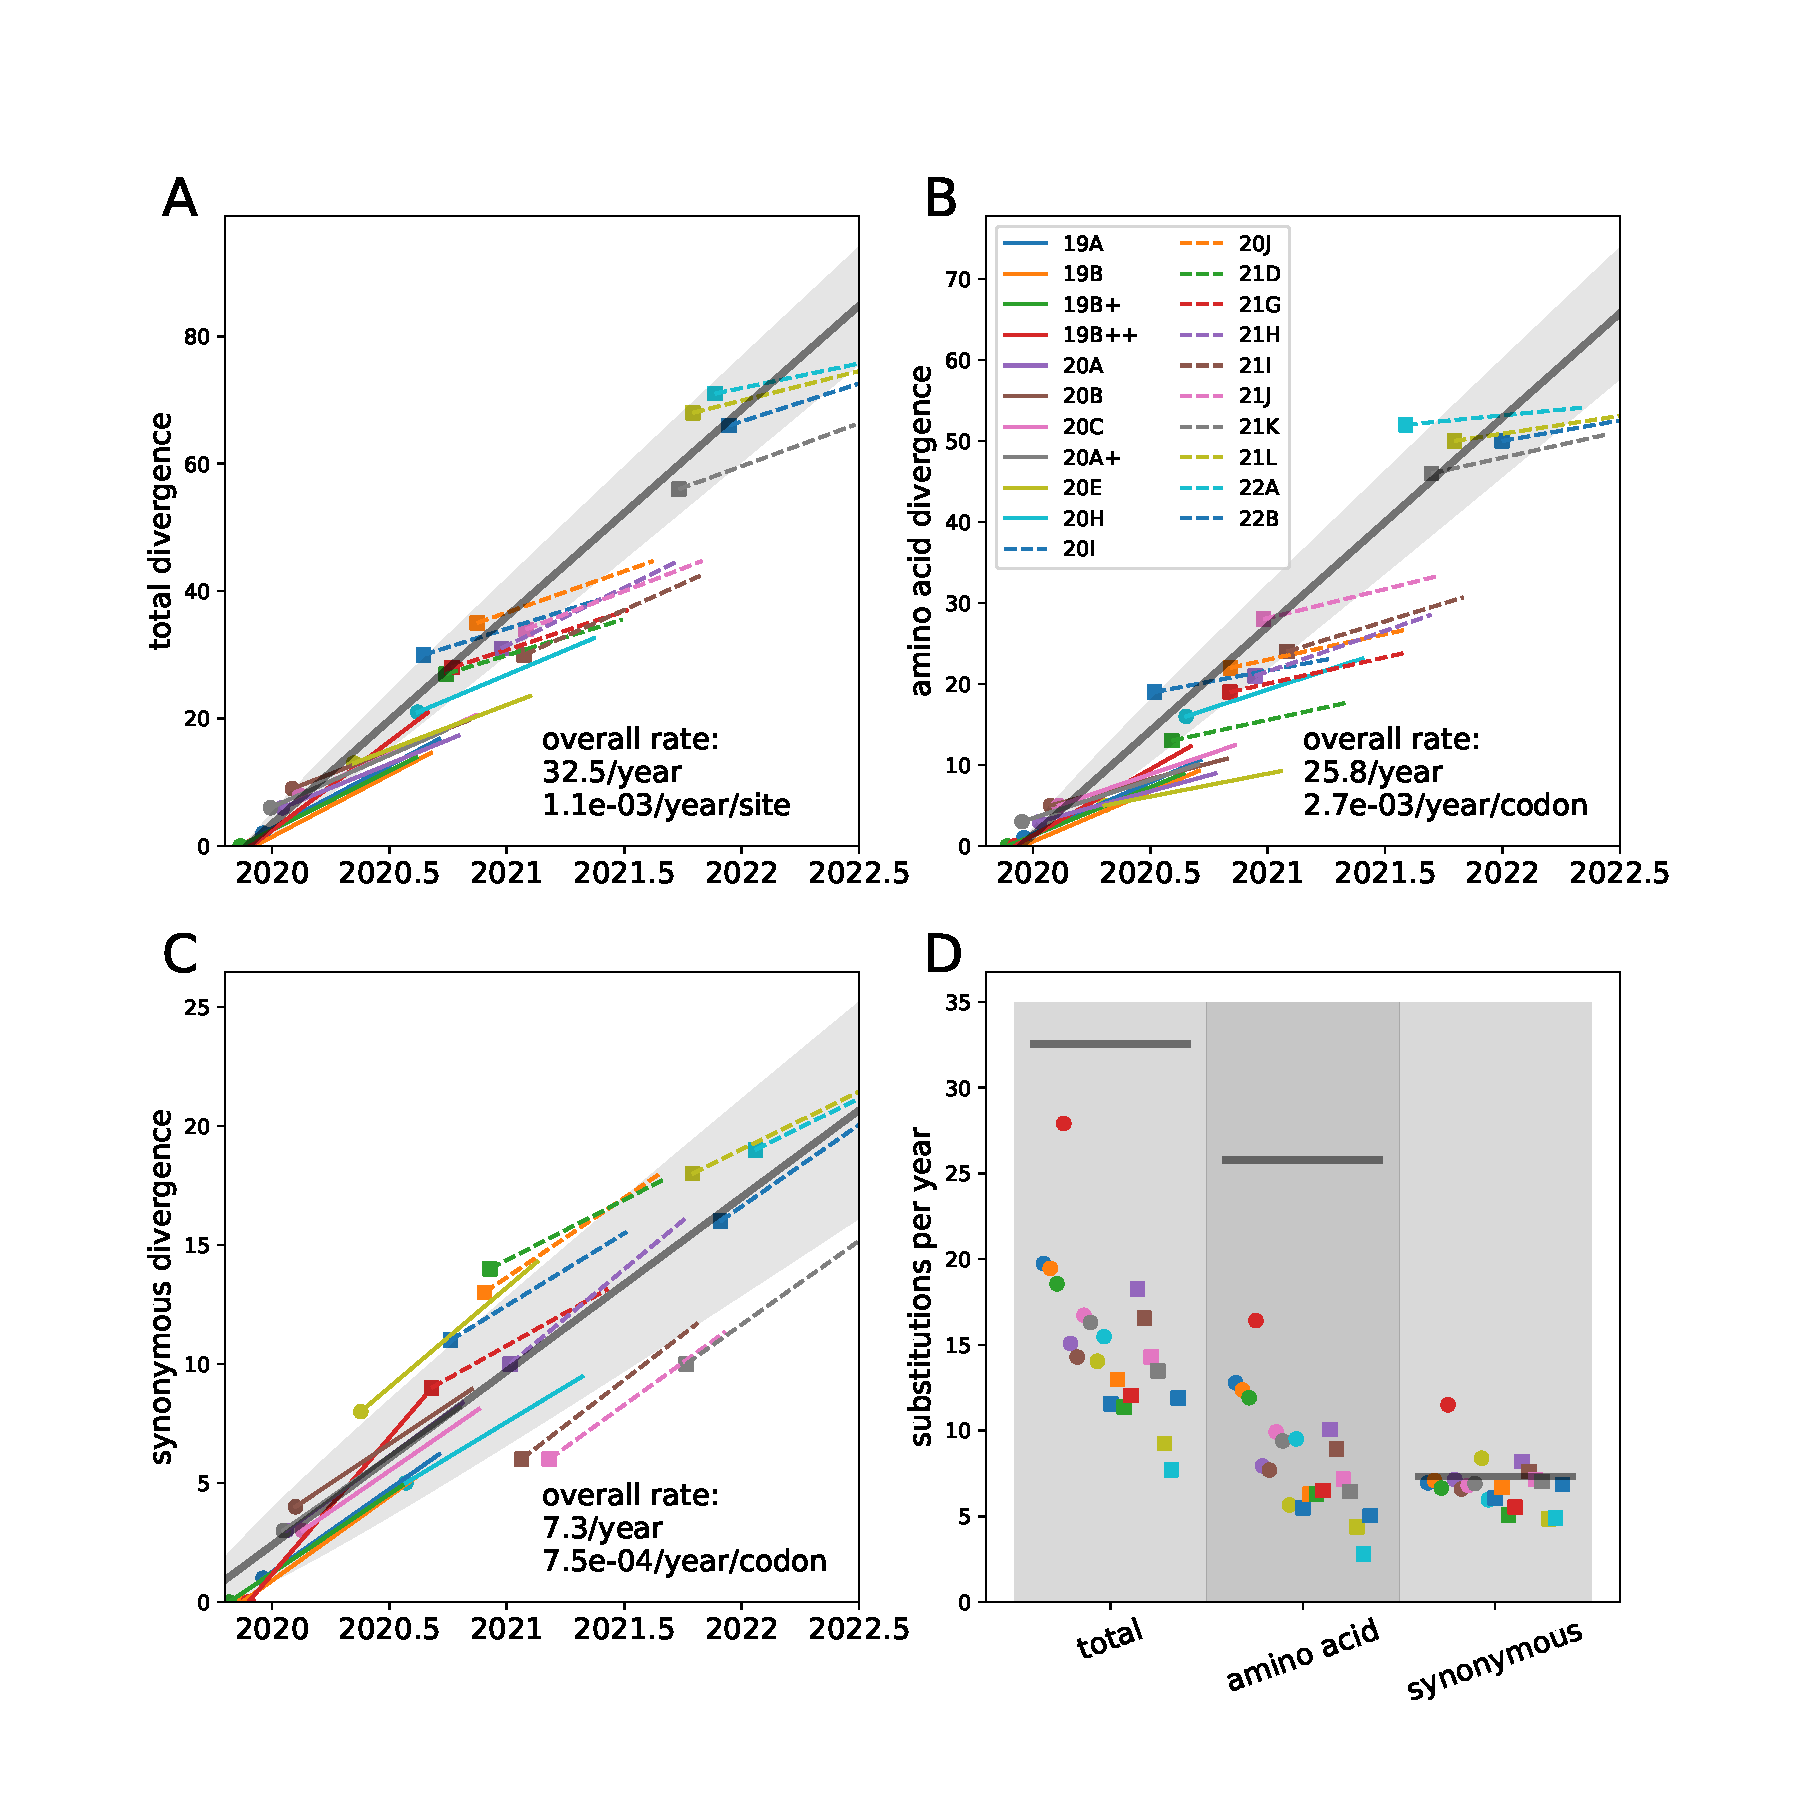
\includegraphics[width=\textwidth]{figures/rate_summary.png}
    \caption[]{{\bf Divergence and evolutionary rates of different Nextstrain clades.} Panels A,B,\&C show the estimated divergence of the founder genotype of each clade (big dot) and the subsequent divergence trend for all nucleotide changes, amino acid changes, and synonymous changes, respectively. In addition, each panel contains a regression of the divergence of clade founders vs time (gray line).
    The standard deviation expected based on Poisson statistics is indicated as shared area.
    Panel D summarizes the individual rate estimate (dots) and compares them to the estimate inter-clade rates (gray lines).
    \label{fig:rate_summary} }
\end{figure*}

Rates of synonymous change are very consistent across variants and also agree with the overall rate of synonymous changes of about 5-8 changes per genome per year.
Rates of non-synonymous changes are much more variable.
Within clades, the rate of non-synonymous changes varies between 5 and 16 changes per year.
Earlier clades are estimated to have larger rates around 10-15 changes per year, while rate estimates for later clade fall  between 3 to 9 changes per year.
In contrast, the inter-clade non-synonymous rate exceeds 25 changes per year.

\begin{table*}
\begin{tabular}{l|rrrrrr}
    \hline
    {\bf clade} &  overall rate $[y^{-1}]$ & aa rate $[y^{-1}]$ &  syn rate $[y^{-1}]$ & overall div. &  aa div. &  syn div. \\
    \hline
      19A &     19.21 &   11.85 &     7.36 &     0 &       0 &        0 \\
      19B &     24.40 &   14.50 &     9.90 &     2 &       1 &        1 \\
      20A &     20.79 &   11.44 &     9.35 &     4 &       2 &        2 \\
      20B &     14.64 &    8.42 &     6.22 &     7 &       4 &        3 \\
      20C &     19.22 &   11.64 &     7.57 &     6 &       4 &        2 \\
     20A+ &     18.48 &   10.26 &     8.22 &     4 &       2 &        2 \\
      20E &     13.77 &    6.04 &     7.73 &    11 &       4 &        7 \\
      20H &     11.16 &    5.22 &     5.94 &    19 &      15 &        4 \\
      20I &     11.65 &    5.77 &     5.88 &    28 &      18 &       10 \\
      20J &     10.93 &    2.66 &     8.28 &    33 &      21 &       12 \\
      21I &     16.53 &    8.88 &     7.65 &    28 &      23 &        5 \\
      21J &     16.20 &    8.19 &     8.00 &    32 &      27 &        5 \\
      21K &     12.74 &    5.41 &     7.34 &    54 &      45 &        9 \\
      21L &      8.66 &    4.67 &     3.99 &    66 &      49 &       17 \\
      22A &      8.46 &    2.92 &     5.55 &    69 &      51 &       18 \\
      22B &     13.78 &    4.13 &     9.65 &    64 &      49 &       15 \\
      \hline
    \end{tabular}
\caption{{\bf Evolutionary rates estimates from root-to-tip regressions for overall nucleotide changes, amino acid changes, and synonymous changes.} \label{tab:rates}}
\end{table*}

\begin{figure}
    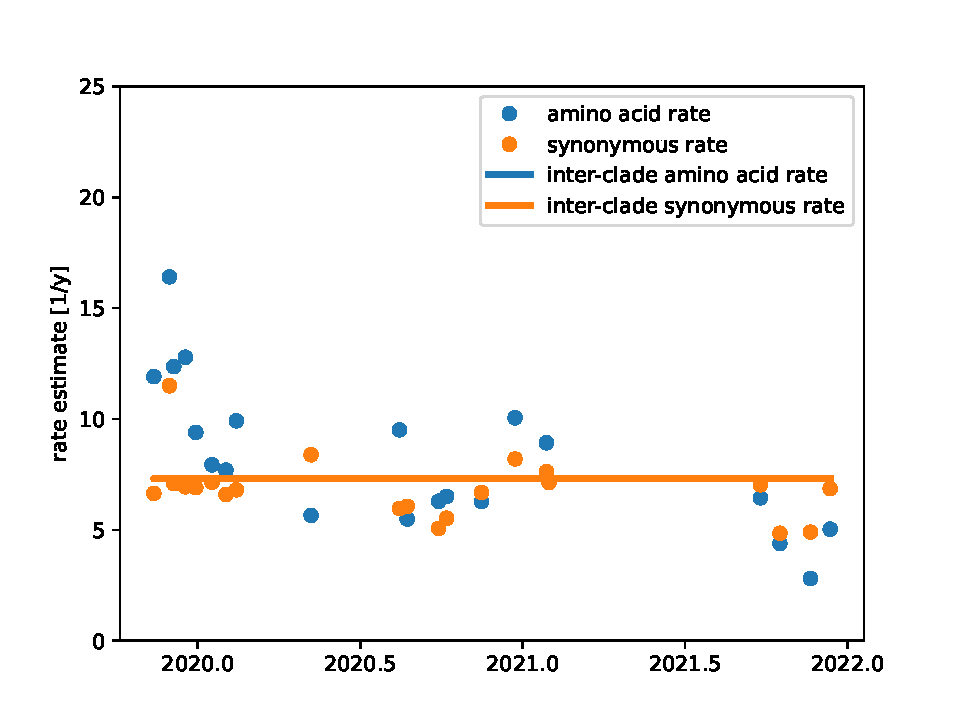
\includegraphics[width=0.5\textwidth]{figures/rate_progression.pdf}
    \caption[]{{\bf Divergence and evolutionary rates of different Nextstrain clades over time.} Synonymous rates estimates are stable in time and fluctuate around the rate estimates for between clades. Non-synonymous rate estimates are highest for clades 19A - 20C.
    \label{fig:rate_progression} }
\end{figure}

The apparent time dependence of non-synonymous rate suggests that at the beginning a large fraction of amino acid changes were beneficial to viral replication, not just the D614G mutation in the spike protein \citep{korber_tracking_2020}.
This applies both to the changes within clades that were ultimately displaced by more successful variants, and inter-variant changes where the fraction of adaptive changes is even higher.
Adaptive evolution complicates phylodynamic analysis, which typically assumes that the mutation process is independent of the spread and epidemiology.
This assumption is true for neutral mutations that occur along every lineage with the same rate.
Adaptive and deleterious mutations, however, affect the ability of the virus to spread.
Deleterious mutations are relatively straightforward to account for: Strongly deleterious mutations don't spread and lead to an evolutionary rate that is smaller than the mutation rates.
Weakly deleterious mutations can spread, but lineages that carry them tend to be short-lived.
A spectrum of mutations with different deleterious effects leads to time dependent effective evolutionary rates \citep{wertheim_purifying_2011}.
The intra-clade rates in Fig.~\ref{fig:rate_progression} are all estimated over a similar time frame and the time dependent rate phenomenon should not apply.

Adaptive evolution, however, is much harder to account for properly and can lead to more dramatic distortions.
Since the number of sites that allow beneficial mutations is small, adaptive evolution tends to be very stochastic.
Unlike neutral evolution, the rate of adaptive evolution depends on the population size and the transmission process.
Epistatic interactions can further steepen the dependence on population size and stochasticity.
Methods to infer emergence dates and locations of the early variants might therefore be biased or over-confident.


\subsection*{Diversification within variants}
The analysis of evolutionary rates above only considers the mean divergence within rates.


\bibliography{bib}
\end{document}
